\section{User Interface Design}
The user interacts with the system through the provided interface. This should contain all relevant information, which are necessary to achieve a specific goal and support her on the way to reach this goal. General user interface approaches from exergame like related work approaches should be compared. Therefore the subsection \textit{\nameref{2_5_1_userInterfacefeedback}} gives an overview on which elements can be used for guiding the user through the system and how feedback can be visualized properly. After that in subsection \textit{\nameref{2_5_2_kinectHIG}} shows how to enhance the user experience on a kinect application with guidelines provided by Microsoft.

\subsection{User interface design for appropriate feedback}\label{2_5_1_userInterfacefeedback}

Important feedback information during the exercise should be placed surrounding the focus point in the peripheral view of the user. Directing the user for correcting her movement can be done in several ways. Basic information about the execution should be given prior to the user for exercise preparation. Surrounding objects can be displayed as arrows, flashing notifications or weighting scale like seen by Garrido et al.~\cite{Garrido2013-zs} in Figure \ref{fig:informationUISurroundingObjects}. 
\begin{figure}[htb]
	\centering
	\begin{minipage}[t]{0.49\linewidth}
		\centering
		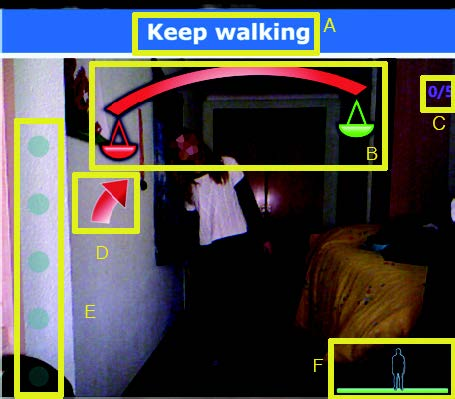
\includegraphics[width=1\linewidth]{Pictures/informationUISurroundingObjects}
		\subcaption{Surrounding elements in the interface}
		\label{fig:informationUISurroundingObjects}
	\end{minipage}
	\hfill
	\begin{minipage}[t]{0.49\linewidth}
		\centering
		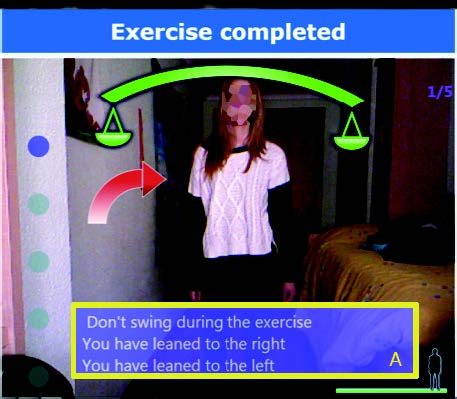
\includegraphics[width=1\linewidth]{Pictures/informationUIFeedbackSummary}
		\subcaption{Completed exercise feedback summary}
		\label{fig:informationUIFeedbackSummary}
	\end{minipage}
	\caption{Interface of a rehabilitation training application~\cite{Garrido2013-zs}}
	\label{fig:informationUIGarrido}
\end{figure}
Additional informations like the current exercise and the state can be displayed outside of the focus space. They should be designed to not distract the user. A feedback summary after the execution can give an useful recap about the exercise for reflection (Figure \ref{fig:informationUIFeedbackSummary}).

Another method is to show the user itself or an avatar that demonstrates the correct performance of the current exercises like in Figure \ref{fig:avatar3DModel} and \ref{fig:avatarUser}. Holsti et al.~\cite{Holsti2013-kn} implemented such a user integration and in user testing they endorse to see themself performing in real time.
\begin{figure}[htb]
	\centering
	\begin{minipage}[t]{0.49\linewidth}
		\centering
		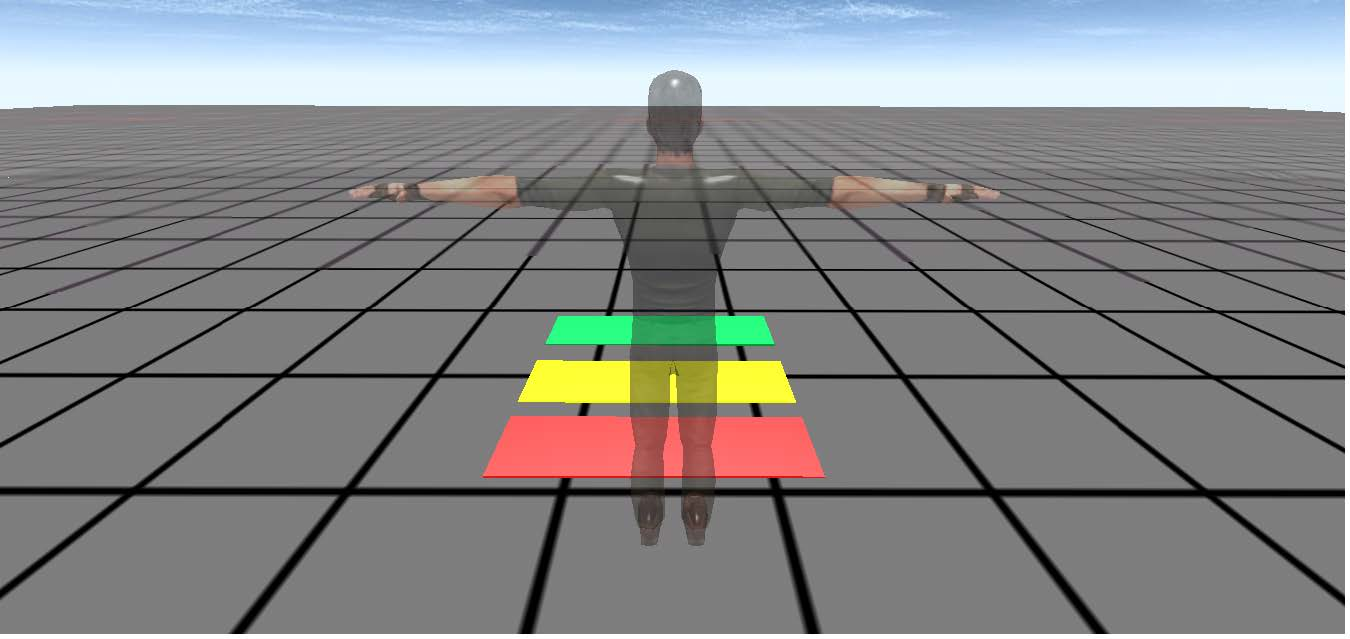
\includegraphics[width=1\linewidth]{Pictures/avatar3DModel}
		\caption{3D Model as avatar~\cite{Estepa2016-oj}}
		\label{fig:avatar3DModel}
	\end{minipage}
	\hfill
	\begin{minipage}[t]{0.49\linewidth}
		\centering
		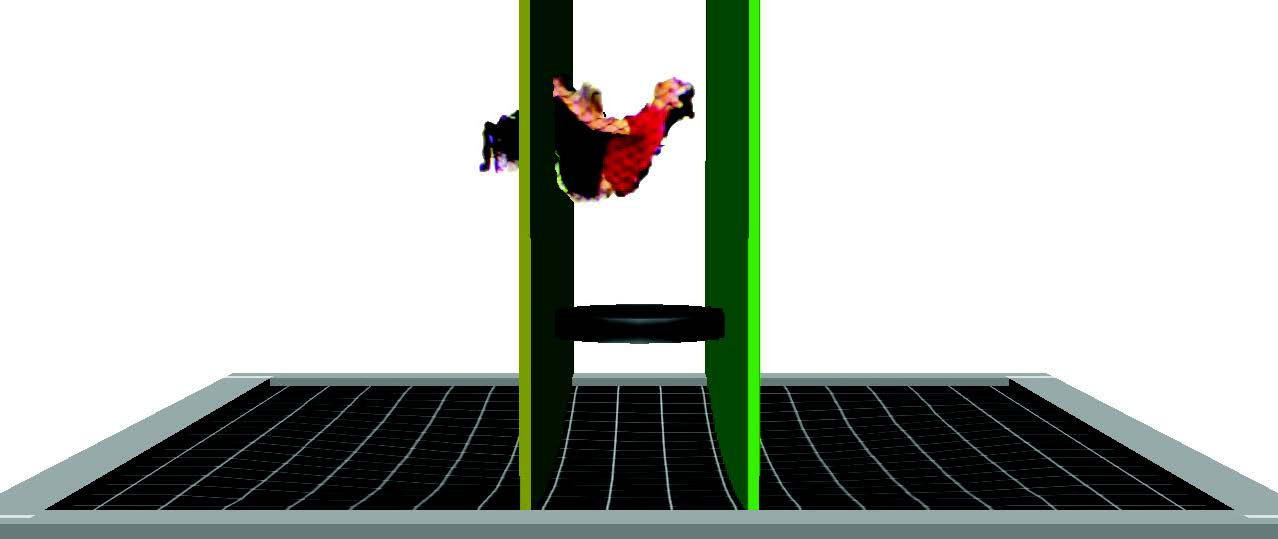
\includegraphics[width=1\linewidth]{Pictures/avatarUser}
		\caption{Rail-time user representation~\cite{Holsti2013-kn}}
		\label{fig:avatarUser}
	\end{minipage}
\end{figure}

The task about the execution has to be clarified. Chang et al.~\cite{Chang2012-hz} provides real time feedback on the performance quality due to a visualised path. If the performance is correct the path will turn green. But if she moves outside the range the path turns red and an arrows guides him into the correct position. Instructions and highlighting objects can help to complete an exercise successfully (Figure \ref{fig:gameUIChang}). If she performs something wrong during the performance e.g. in the slacklining case corresponding body parts could be highlighted.
\begin{figure}[htb]
	\centering
	\begin{minipage}[t]{0.49\linewidth}
		\centering
		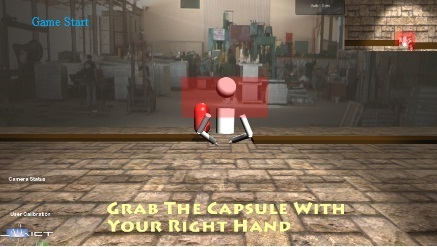
\includegraphics[width=1\linewidth]{Pictures/gameInstruction}
		\subcaption{Instruction to the game}
		\label{fig:gameInstruction}
	\end{minipage}
	\hfill
	\begin{minipage}[t]{0.49\linewidth}
		\centering
		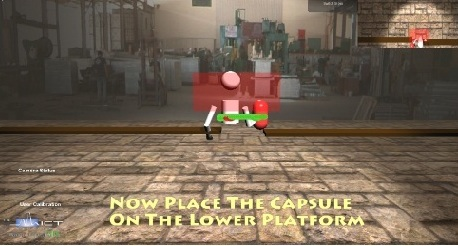
\includegraphics[width=1\linewidth]{Pictures/gameHighlighting}
		\subcaption{Green indicator for correct performance}
		\label{fig:gameHighlighting}
	\end{minipage}
	\caption{User interface of a rehabilitational application~\cite{Chang2012-hz}}
	\label{fig:gameUIChang}
\end{figure}

\subsection{Kinect for Windows - Human Interface Guidelines}\label{2_5_2_kinectHIG}
Microsoft itself offers Human-Interface-Guidelines (HIG) for developer and designer that describes several techniques of certain areas for developing a kinect application~\cite{MicrosoftHIG2014-mh}. It provides a quick introduction into the Kinect itself, design principles for interactions regarding gesture and voice, techniques on teaching complex gestures, and how to visualize appropriate feedback. Also which interactions should be used for a specific action. Therefore developer may follow this general standard to support their end-user. In the following general principles of the guideline will be discussed on which the interactive slackline system will rely on to enhance the user experience. 
%The general design principles are that the application should be context-aware, make the user confident, choosing the right input method and to conduct user tests. 

\subsubsection{Basic design principles}
Context-awareness delivers the best user experience e.g. controls should be placed where user would expect them to be and interactions should be appropriate for the environment. It is important that the user feel confident by designing interactions simple and easy to learn. User will choose an input that take the least effort for the given goal. Therefore the input method should match its purpose, be reliable, consistent, and convenient. Conducting user test helps to improve the system. Not each person will use the system the same way and minor adjustments can make a huge difference in the understanding of the usage.

\subsubsection{Visual and audio feedback}
Giving the user constant feedback helps her to know what is happening. In general appropriate feedback should show if the sensor is ready, she is visible and engaging with the Kinect, and so on (Figure \ref{fig:hciGuidelinesFeedbackCursor}). Regarding this a combination of visual as well as audio feedback results in a better experience, e.g. clicking a button changes its visual state and provides an audio signal (Figure \ref{fig:hciGuidelinesFeedbackControl}).
\begin{comment}
\begin{figure}[htb]
	\centering
	\begin{minipage}[t]{0.45\linewidth}
		\centering
		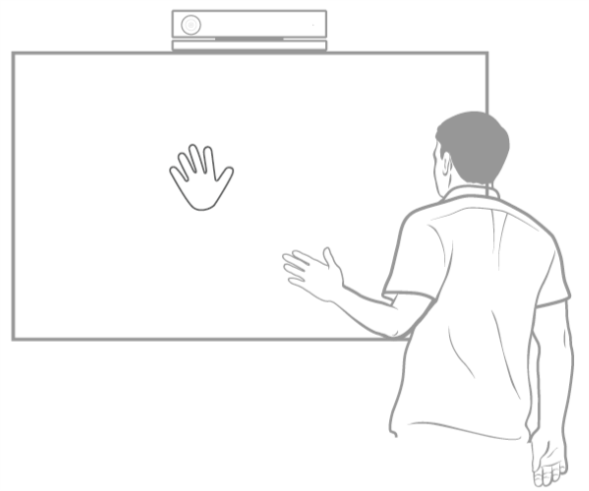
\includegraphics[width=0.5\linewidth]{Pictures/hciGuidelinesFeedbackCursor}
		\caption{Hand cursor visualizes the engagement and readiness of the system~\cite{MicrosoftHIG2014-mh}}
		\label{fig:hciGuidelinesFeedbackCursor}
	\end{minipage}
	\hfill
	\begin{minipage}[t]{0.45\linewidth}
		\centering
		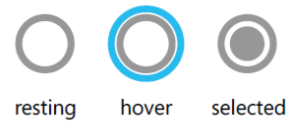
\includegraphics[width=0.5\linewidth]{Pictures/hciGuidelinesFeedbackControl}
		\caption{Different states of UI controls~\cite{MicrosoftHIG2014-mh}}
		\label{fig:hciGuidelinesFeedbackControl}
	\end{minipage}
\end{figure}
\end{comment}
\begin{figure}[htb]
	\centering
	\begin{minipage}[t]{0.45\linewidth}
		\centering
		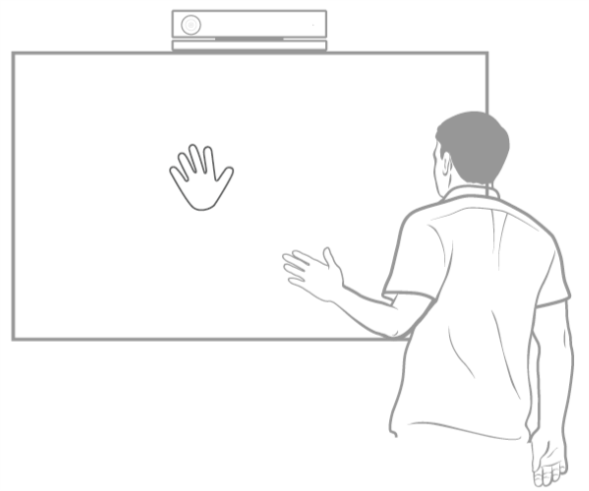
\includegraphics[width=0.5\linewidth]{Pictures/hciGuidelinesFeedbackCursor}
		\subcaption{Hand cursor visualizes the engagement and readiness of the system}
		\label{fig:hciGuidelinesFeedbackCursor}
	\end{minipage}
	\hfill
	\begin{minipage}[t]{0.45\linewidth}
		\centering
		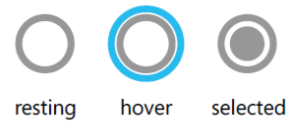
\includegraphics[width=0.5\linewidth]{Pictures/hciGuidelinesFeedbackControl}
		\subcaption{Different states of UI controls}
		\label{fig:hciGuidelinesFeedbackControl}
	\end{minipage}
	\caption{Feedback methods~\cite{MicrosoftHIG2014-mh}}
	\label{fig:hciGuidelinesFeedback}
\end{figure}

The most important part for complex gestures is the progress indicator described in this guideline. It supports the user if she has to hold a position, as well as if an amount of frequent repetitions have to be performed. Clear and prominent visuals should be used to show the entire progression (Figure \ref{fig:visualFeedbackIndicator}). If a user has to copy a specific movement an avatar or animation can be shown, before or during the movement, like in Figure \ref{fig:visualFeedbackAvatar}.
\begin{figure}[htb]
	\centering
	\begin{minipage}[t]{0.49\linewidth}
		\centering
		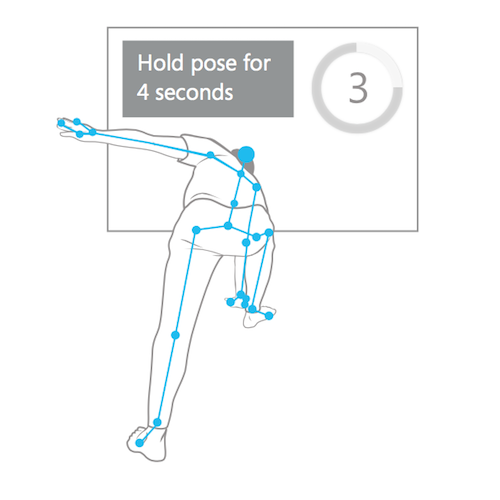
\includegraphics[width=0.9\linewidth]{Pictures/2_4_visualFeedbackIndicator}
		\subcaption{Repetition and time length indicators}
		\label{fig:visualFeedbackIndicator}
	\end{minipage}
	\hfill
	\begin{minipage}[t]{0.49\linewidth}
		\centering
		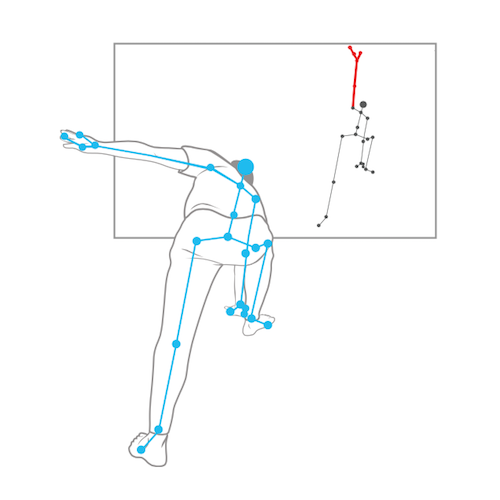
\includegraphics[width=0.9\linewidth]{Pictures/2_4_visualFeedbackAvatar}
		\subcaption{Avatar that shows correct movement and wrong body parts are highlighted}
		\label{fig:visualFeedbackAvatar}
	\end{minipage}
	\caption{Feedback indicator and movement visualization as an avatar~\cite{MicrosoftHIG2014-mh}}
	\label{fig:hciGuidelinesIndicatorAvatar}
\end{figure}

\subsubsection{Clarification}
The user may interpret interactions with the system differently from others. Therefore the system should explain clearly what the user has to do, e.g. \textit{"Raise one hand above your head"} instead of just \textit{"Raise your hand"}. The cognitive load of the user should be kept low and not exceed a number of six gestures, such that she easily remembers the actions. The system has a set of three basic interaction techniques, which fits in this range.

\subsubsection{User viewer}
A small scene viewer shows the range in which the user can move and is recognized by the Kinect. It displays a mirror like view in which the user can see a silhouette of herself and the constraints of the Kinect device, like in figure \ref{fig:higUserViewer}.
\begin{figure}[htb]
	\centering
	\begin{minipage}[t]{1\linewidth}
		\centering
		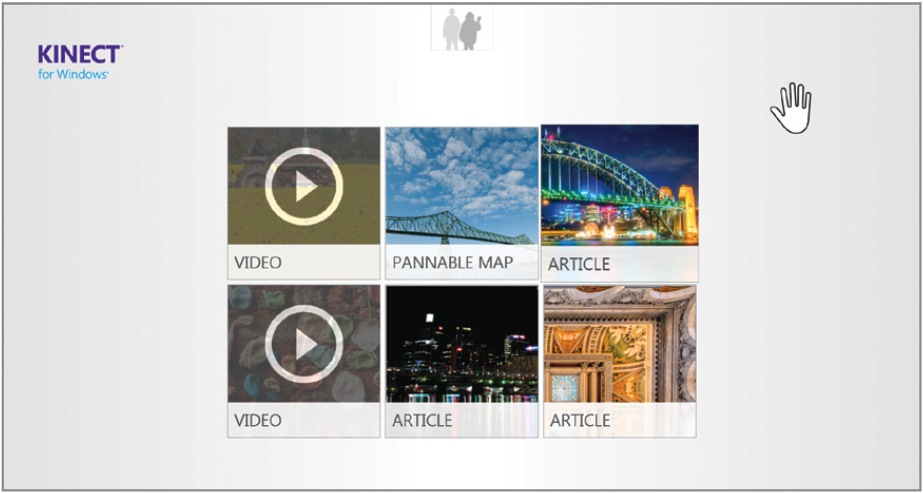
\includegraphics[width=0.6\linewidth]{Pictures/higUserViewer}
		\caption{User Viewer on top~\cite{MicrosoftHIG2014-mh}}
		\label{fig:higUserViewer}
	\end{minipage}
\end{figure}

\subsubsection{Learning interaction methods}
The application should teach the user how to proper interact with it right from the beginning with an introduction tutorial. An interaction itself should rely on the real world, which can help the user to be more familiar with the product, than learning unknown gestures (Figure \ref{fig:hciGuidelinesDynamicGesture}). Also biliteral interaction support should be applied to cover both possibilities for left- and right-handed people.
\begin{figure}[htb]
	\centering
	\begin{minipage}[t]{1\linewidth}
		\centering
		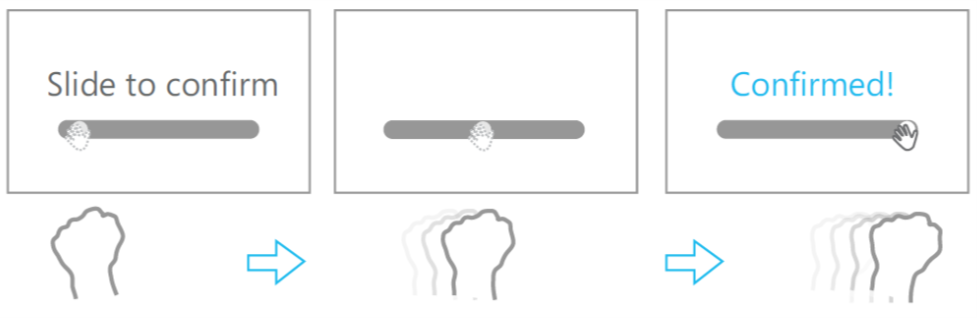
\includegraphics[width=0.6\linewidth]{Pictures/hciGuidelinesDynamicGesture}
		\caption{Direct manipulation of a slider with intuitive interaction~\cite{MicrosoftHIG2014-mh}}
		\label{fig:hciGuidelinesDynamicGesture}
	\end{minipage}
\end{figure}

\subsubsection{Teaching complex gestures / exercises}
Executing gestures is a core functionality in the slacklining assistance system. For new gestures, especially complex ones, the application should provide a tutorial that teaches and shows the user on how to execute or accomplish the gesture properly. When performing the gesture a visual indicator (a hint, animation, or notification) should acknowledge if the gesture is executed and when it is completed. (Figure \ref{fig:hciGuidelinesTeachingMethods}).
\begin{figure}[htb]
	\centering
	\begin{minipage}[t]{1\linewidth}
		\centering
		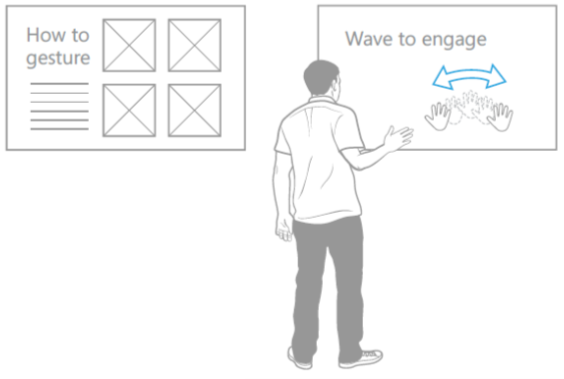
\includegraphics[width=0.4\linewidth]{Pictures/hciGuidelinesTeachingMethods}
		\caption{Teaching new gestures~\cite{MicrosoftHIG2014-mh}}
		\label{fig:hciGuidelinesTeachingMethods}
	\end{minipage}
\end{figure}

\subsubsection{Element sizing}
The system will rely on the guidelines and match the button sizing regarding the screen resolution to keep reliability on interaction. This is a size of 208 by 208px in a resolution of 1920x1080 pixel. As recommended a tile button style will be used which are a good baseline where the user can hit them accurately and read the button text.

\subsubsection{Physical interaction zone}
This zone ensures that the user is able to reach anything in a comfortable range. In the application it is constrained by the joints of the shoulders to the hips of the opposite site of the interaction hand. It is designed like seen in figure \ref{fig:higPHIZ} to have a better understanding.
\begin{figure}[htb]
	\centering
	\begin{minipage}[t]{1\linewidth}
		\centering
		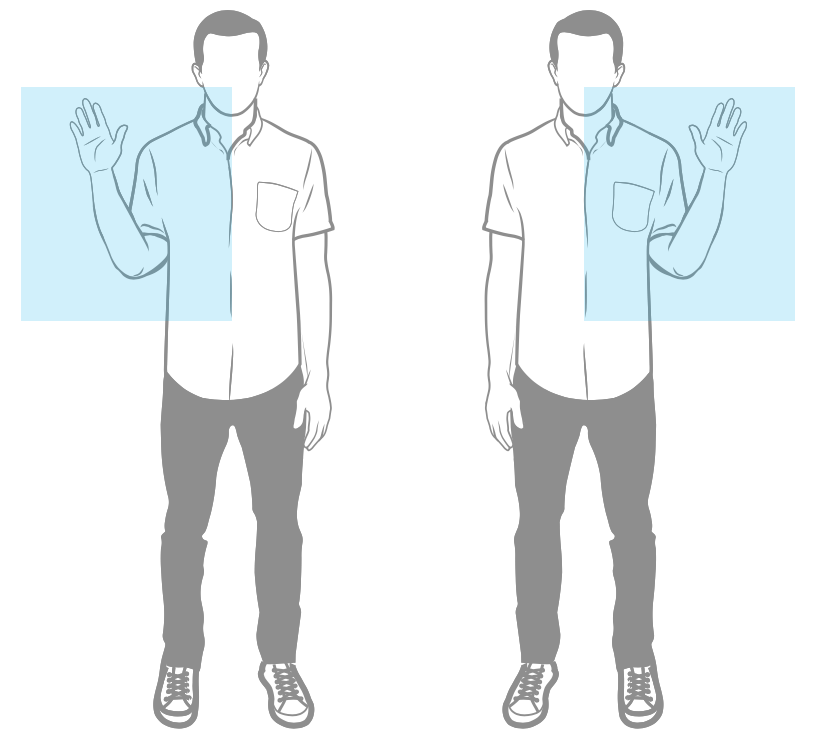
\includegraphics[width=0.32\linewidth]{Pictures/higPHIZ}
		\caption{Physical interaction zone~\cite{MicrosoftHIG2014-mh}}
		\label{fig:higPHIZ}
	\end{minipage}
\end{figure}

\begin{comment}
- System should provide a user view, such that the user knows the constraints of the kinect tracking area --> should be small if interacting in menu and big if needed in execution for example
\\- Audio feedback (success/failing)
\\- Big buttons/selectable elements
\\- Button state changes --> visualize
\\- \todo{picture of key elements from Kinect HIG}

- \todo{maybe combine interaction with key elements of a kinect application}
\end{comment}


Summarizing the user interface should not distract the slacker but support him. Only necessary and useful information have to be displayed during the exercise. Providing an introduction and useful tips can help to give an understanding of the exercise. An avatar or animation is a good alternative to make clear how to perform an exercise. The system should also rely on Microsoft human interface guidelines, which provides design tips and serves as a reference to build user friendly applications.
